\documentclass[aspectratio=169,11pt]{beamer}
\usepackage[T1]{fontenc}
\usepackage{lmodern,amsmath,amssymb,mathtools,bm,booktabs,array,graphicx,tikz}
\usetikzlibrary{arrows.meta,positioning,calc,decorations.pathreplacing,patterns}
\definecolor{ink}{HTML}{17344D}\definecolor{accent}{HTML}{087E8B}\definecolor{pale}{HTML}{EDF5F5}\definecolor{gold}{HTML}{AD6B19}
\providecommand{\dd}{\,\mathrm{d}}\providecommand{\R}{\mathbb{R}}
\providecommand{\E}{\mathbb{E}}\providecommand{\Var}{\operatorname{Var}}
\providecommand{\Cov}{\operatorname{Cov}}\providecommand{\diag}{\operatorname{diag}}
\providecommand{\norm}[1]{\left\lVert#1\right\rVert}
\providecommand{\abs}[1]{\left|#1\right|}
\usefonttheme{professionalfonts}
\setbeamercolor{normal text}{fg=black,bg=white}
\setbeamercolor{frametitle}{fg=ink,bg=white}
\setbeamercolor{title}{fg=ink}\setbeamercolor{structure}{fg=accent}
\setbeamercolor{block title}{fg=ink,bg=pale}\setbeamercolor{block body}{fg=black,bg=pale!40}
\setbeamercolor{alerted text}{fg=accent}
\setbeamerfont{frametitle}{size=\Large,series=\bfseries}
\setbeamerfont{title}{size=\LARGE,series=\bfseries}
\setbeamertemplate{navigation symbols}{}
\setbeamersize{text margin left=.7cm,text margin right=.7cm}
\setbeamertemplate{frametitle}{\vspace{.18cm}\insertframetitle\par\vspace{.1cm}{\color{accent}\hrule height .6pt}\vspace{.12cm}}
\newcommand{\notestarget}{notes.pdf}\newcommand{\noteslabel}{Notes}
\setbeamertemplate{footline}{\hspace{.7cm}\color{ink}\scriptsize Computational Cardiology\quad\href{\notestarget}{\noteslabel}\hfill\insertframenumber\,/\,\inserttotalframenumber\hspace{.7cm}\vspace{.18cm}}
\setbeamercovered{invisible}
\hypersetup{pdfauthor={Zan Ahmad},pdftitle={Circulatory models and parameter identifiability},pdfpagemode=UseNone}
\begin{document}
\begin{frame}[plain]\vfill
{\small\color{accent} Computational Cardiology \quad Lecture 1}\par\medskip
{\raggedright\hyphenpenalty=10000\exhyphenpenalty=10000\LARGE\bfseries\color{ink} Circulatory models and parameter identifiability}\par\bigskip
Zan Ahmad\par\smallskip
{\small Fall 2024}\par\vfill\end{frame}
\renewcommand{\notestarget}{notes.pdf\#note-model-resolution-and-measurable-quantities}
\begin{frame}[t,fragile,label=slide-states-and-observations]{States and observations}
\[\dot x=F(x,\vartheta,u),\qquad y=H(x,\vartheta,u).\]\pause{}
The state determines how the model continues. The observation map determines what the experiment can distinguish.
\end{frame}
\renewcommand{\notestarget}{notes.pdf\#note-model-resolution-and-measurable-quantities}
\begin{frame}[t,fragile,label=slide-resolution-follows-the-observable]{Resolution follows the observable}
\begin{align*}
\text{mean perfusion}&\longrightarrow\overline Q,\\
\text{valve timing}&\longrightarrow P_i(t),\ q_{ij}(t),\\
\text{wall mechanics}&\longrightarrow \sigma(x,t).
\end{align*}\pause{}
A compartment volume does not contain a spatial stress distribution.
\end{frame}
\renewcommand{\notestarget}{notes.pdf\#note-a-closed-circulation-as-a-directed-network}
\begin{frame}[t,fragile,label=slide-the-two-pump-circuit]{The two-pump circuit}
\centering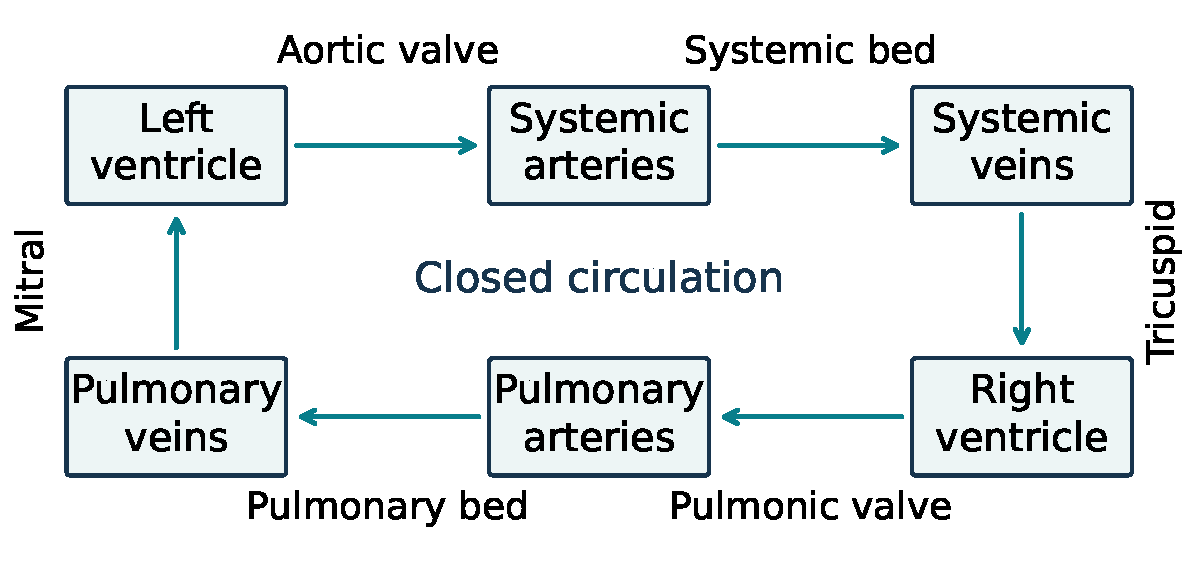
\includegraphics[width=.98\linewidth,height=.52\textheight,keepaspectratio]{presentation-figures/circulation-map-panel-1.pdf}\par\raggedright
\pause{}
The closed network contains two ventricles and four vascular storage regions. Atrial storage is not a separate state in this grouping.
\end{frame}
\renewcommand{\notestarget}{notes.pdf\#note-a-closed-circulation-as-a-directed-network}
\begin{frame}[t,fragile,label=slide-the-incidence-matrix]{The incidence matrix}
For each directed edge, put $-1$ at its donor and $+1$ at its receiver.
\[\dot{\boldsymbol V}=B\boldsymbol q.\]\pause{}
Every column sums to zero: $\boldsymbol1^{\mathsf T}B=0$.
\end{frame}
\renewcommand{\notestarget}{notes.pdf\#note-a-closed-circulation-as-a-directed-network}
\begin{frame}[t,fragile,label=slide-conservation-of-total-volume]{Conservation of total volume}
\[\frac{\mathrm d}{\mathrm dt}\sum_iV_i=\boldsymbol1^{\mathsf T}B\boldsymbol q=0.\]\pause{}
With an external source $s$, the right-hand side becomes $\boldsymbol1^{\mathsf T}s$. The boundary determines the conserved quantity.
\end{frame}
\renewcommand{\notestarget}{notes.pdf\#note-pressure-storage-and-physical-units}
\begin{frame}[t,fragile,label=slide-flow-and-compliant-storage]{Flow and compliant storage}
\[q_{ij}=\frac{P_i-P_j}{R_{ij}},\qquad V_i=V_{0i}+C_i(P_i-P_{{\rm ext},i}).\]\pause{}
Fluid pressure difference drives flow. Transmural pressure determines storage.
\end{frame}
\renewcommand{\notestarget}{notes.pdf\#note-pressure-storage-and-physical-units}
\begin{frame}[t,fragile,label=slide-dimensions-of-the-constitutive-laws]{Dimensions of the constitutive laws}
\[[R]=\frac{\mathrm{mmHg}\,\mathrm{min}}{\mathrm L},\qquad [C]=\frac{\mathrm L}{\mathrm{mmHg}}.\]\pause{}
\[[RC]=\mathrm{min}.\]
A pressure gauge shift preserves storage only when the exterior reference shifts consistently.
\end{frame}
\renewcommand{\notestarget}{notes.pdf\#note-mean-flow-as-an-observation-map}
\begin{frame}[t,fragile,label=slide-transport-over-repeated-beats]{Transport over repeated beats}
For $n$ identical beats in $T$ minutes,
\[\overline Q=\frac{n\,SV}{1000T}=\frac{F\,SV}{1000}.\]\pause{}
For unequal beats, replace $n\,SV$ by $\sum_k SV_k$.
\end{frame}
\renewcommand{\notestarget}{notes.pdf\#note-mean-flow-as-an-observation-map}
\begin{frame}[t,fragile,label=slide-a-mean-flow-calculation]{A mean-flow calculation}
\[F=80\ \mathrm{min}^{-1},\qquad SV=75\ \mathrm{mL},\qquad \Delta P=90\ \mathrm{mmHg}.\]\pause{}
\[\overline Q=6\ \mathrm{L/min},\qquad R_{\rm eff}=\frac{90}{6}=15\ \mathrm{mmHg\,min/L}.\]
\end{frame}
\renewcommand{\notestarget}{notes.pdf\#note-parameter-symmetries-and-local-identifiability}
\begin{frame}[t,fragile,label=slide-an-exact-parameter-symmetry]{An exact parameter symmetry}
\[H(F,SV)=\frac{F\,SV}{1000},\qquad H(aF,SV/a)=H(F,SV),\quad a>0.\]\pause{}
The same mean flow corresponds to infinitely many positive parameter pairs.
\end{frame}
\renewcommand{\notestarget}{notes.pdf\#note-parameter-symmetries-and-local-identifiability}
\begin{frame}[label=slide-a-level-set-of-the-observation-map-figure]{One mean-flow observation leaves many possibilities}
\centering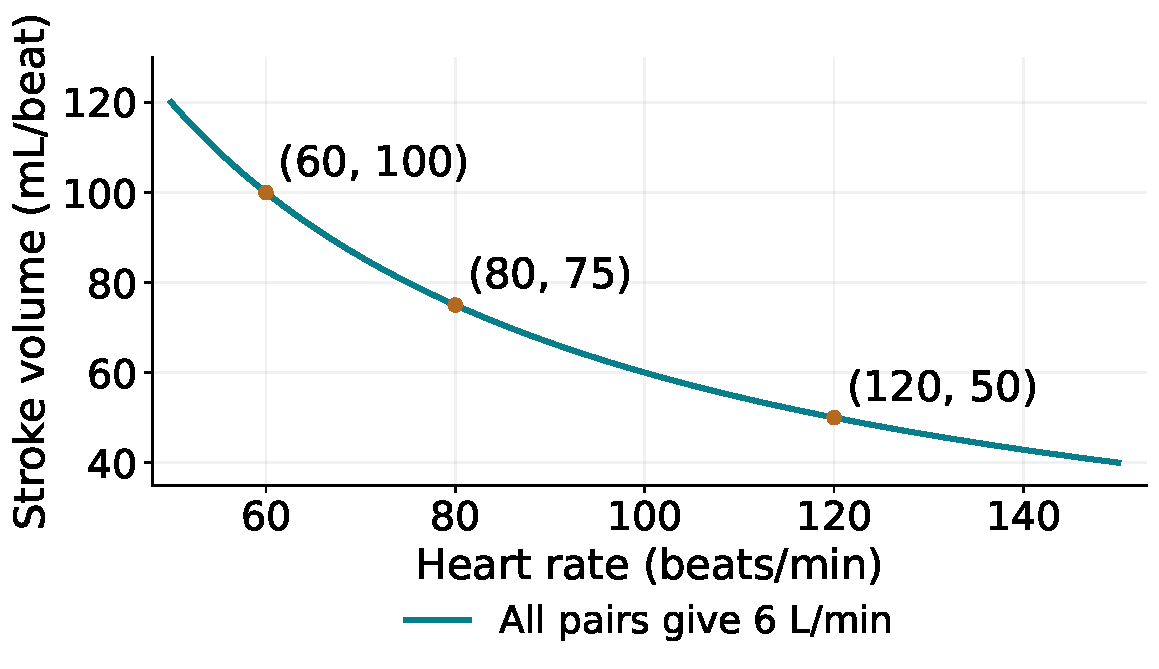
\includegraphics[width=.98\linewidth,height=.69\textheight,keepaspectratio]{presentation-figures/flow-identifiability-panel-1.pdf}\end{frame}
\renewcommand{\notestarget}{notes.pdf\#note-parameter-symmetries-and-local-identifiability}
\begin{frame}[t,fragile,label=slide-a-level-set-of-the-observation-map]{A level set of the observation map}
\[SV=\frac{1000Q_0}{F}.\]
The pairs $(60,100)$, $(80,75)$ and $(120,50)$ all lie on the $Q_0=6$ level set.
\end{frame}
\renewcommand{\notestarget}{notes.pdf\#note-parameter-symmetries-and-local-identifiability}
\begin{frame}[t,fragile,label=slide-the-unobservable-perturbation]{The unobservable perturbation}
\[\delta Q=\frac{SV\,\delta F+F\,\delta SV}{1000}.\]\pause{}
\[DH\begin{pmatrix}F\\-SV\end{pmatrix}=0,\qquad
\frac{\delta F}{F}=-\frac{\delta SV}{SV}.\]
Opposite relative changes cancel to first order.
\end{frame}
\renewcommand{\notestarget}{notes.pdf\#note-independent-observations-and-model-error}
\begin{frame}[t,fragile,label=slide-adding-an-independent-measurement]{Adding an independent measurement}
\[\widetilde H(F,SV)=\begin{pmatrix}F\,SV/1000\\F\end{pmatrix}.\]\pause{}
\[\det D\widetilde H=-\frac F{1000}\ne0\quad(F>0).\]
Measured rate removes this particular ambiguity.
\end{frame}
\renewcommand{\notestarget}{notes.pdf\#note-independent-observations-and-model-error}
\begin{frame}[t,fragile,label=slide-uncertainty-in-inferred-stroke-volume]{Uncertainty in inferred stroke volume}
\[SV=\frac{1000Q}{F}.\]\pause{}
\[\frac{\delta SV}{SV}\simeq\frac{\delta Q}{Q}-\frac{\delta F}{F}.\]
Identifiability supplies a unique local inverse; measurement precision determines how uncertain that inverse remains.
\end{frame}
\renewcommand{\notestarget}{notes.pdf\#note-independent-observations-and-model-error}
\begin{frame}[t,fragile,label=slide-information-retained-by-the-model]{Information retained by the model}
Mean flow and measured rate determine stroke volume under the repeated-cycle assumption.\pause{}

They do not determine a ventricular pressure waveform, valve leakage or a spatial stress field. Those quantities require additional states and observations.
\end{frame}
\end{document}
